\clearpage
\appendix


\section{Detailed Error Bound Derivation}
\label{app:full_error_bound}

% 为了使用 \begin{proof} ... \end{proof} 环境, 请在序言部分引入 amsthm 宏包
% \usepackage{amsthm}
% \newtheorem{lemma}{Lemma}

In this section, we provide the detailed proofs for the two key approximations that underpin the LongFlow method, justifying the claims made in Section \ref{sec:error_bound_final}. Our goal is to bound the total error \( \mathcal{E}^i = \left| \left\| \mathbf{o}_{t+1} - \mathbf{o}_{t+1}^{(\setminus i)} \right\|^2 - \left\| \mathbf{c}_t^i \right\|^2 \right| \), which we decompose using the triangle inequality:
\begin{equation}
\resizebox{\columnwidth}{!}{$
    \mathcal{E}^i \le \underbrace{\left| \left\| \mathbf{o}_{t+1} - \mathbf{o}_{t+1}^{(\setminus i)} \right\|^2 - \left\| \mathbf{c}_{t+1}^i \right\|^2 \right|}_{\text{Error from Denominator Approx.}} + \underbrace{\left| \left\| \mathbf{c}_{t+1}^i \right\|^2 - \left\| \mathbf{c}_t^i \right\|^2 \right|}_{\text{Error from Query Drift}}.
$}
\end{equation}
We now derive explicit bounds for each of these two error terms.

\subsection{Bounding the Error from the Denominator Approximation}

This error arises from approximating the true change in attention output, \( \Delta\mathbf{o}_{t+1} = \mathbf{o}_{t+1} - \mathbf{o}_{t+1}^{(\setminus i)} \), with the contribution vector \( \mathbf{c}_{t+1}^i = \alpha_{t+1}^i \mathbf{v}^i \). We now derive an exact expression for the remainder term \( \mathbf{R}_{t+1}^i = \Delta\mathbf{o}_{t+1} - \mathbf{c}_{t+1}^i \).

First, let us expand the terms. The original attention output is a sum over all \(t\) historical tokens, while the output after eviction is a sum over the remaining \(t-1\) tokens with re-normalized attention weights:
\begin{align*}
    \mathbf{o}_{t+1} &= \sum_{j=1}^{t} \alpha_{t+1}^j \mathbf{v}^j = \alpha_{t+1}^i \mathbf{v}^i + \sum_{j \neq i} \alpha_{t+1}^j \mathbf{v}^j \\
    \mathbf{o}_{t+1}^{(\setminus i)} &= \sum_{j \neq i} \alpha_{t+1}^{j, (\setminus i)} \mathbf{v}^j
\end{align*}
Substituting these into the definition of the remainder term:
% \begin{align*}
%     \mathbf{R}_{t+1}^i &= \Delta\mathbf{o}_{t+1} - \mathbf{c}_{t+1}^i \\
%     &= \left( \mathbf{o}_{t+1} - \mathbf{o}_{t+1}^{(\setminus i)} \right) - \mathbf{c}_{t+1}^i \\
%     &= \left( \left( \alpha_{t+1}^i \mathbf{v}^i + \sum_{j \neq i} \alpha_{t+1}^j \mathbf{v}^j \right) - \left( \sum_{j \neq i} \alpha_{t+1}^{j, (\setminus i)} \mathbf{v}^j \right) \right) - \alpha_{t+1}^i \mathbf{v}^i \\
%     &= \sum_{j \neq i} \left( \alpha_{t+1}^j - \alpha_{t+1}^{j, (\setminus i)} \right) \mathbf{v}^j.
% \end{align*}
\begin{align*}
    \mathbf{R}_{t+1}^i &= \Delta\mathbf{o}_{t+1} - \mathbf{c}_{t+1}^i \\
    &= \left( \mathbf{o}_{t+1} - \mathbf{o}_{t+1}^{(\setminus i)} \right) - \mathbf{c}_{t+1}^i \\
    &= \biggl( \alpha_{t+1}^i \mathbf{v}^i + \sum_{j \neq i} \alpha_{t+1}^j \mathbf{v}^j \biggr) \\
    &\quad - \biggl( \sum_{j \neq i} \alpha_{t+1}^{j, (\setminus i)} \mathbf{v}^j \biggr) - \alpha_{t+1}^i \mathbf{v}^i \\
    &= \sum_{j \neq i} \left( \alpha_{t+1}^j - \alpha_{t+1}^{j, (\setminus i)} \right) \mathbf{v}^j.
\end{align*}

The key is to relate the new weights \( \alpha_{t+1}^{j, (\setminus i)} \) to the old weights \( \alpha_{t+1}^j \). The new weights are re-normalized over a smaller set of tokens:
% \[
%     \alpha_{t+1}^{j, (\setminus i)} = \frac{\exp(s_{t+1}^j)}{\sum_{l \neq i} \exp(s_{t+1}^l)} = \frac{\exp(s_{t+1}^j)}{Z_{t+1} - \exp(s_{t+1}^i)} = \frac{\exp(s_{t+1}^j)/Z_{t+1}}{(Z_{t+1} - \exp(s_{t+1}^i))/Z_{t+1}} = \frac{\alpha_{t+1}^j}{1 - \alpha_{t+1}^i}.
% \]
\begin{equation}
\begin{split}
    \alpha_{t+1}^{j, (\setminus i)} &= \frac{\exp(s_{t+1}^j)}{\sum_{l \neq i} \exp(s_{t+1}^l)} \\
    &= \frac{\exp(s_{t+1}^j)}{Z_{t+1} - \exp(s_{t+1}^i)} \\
    &= \frac{\exp(s_{t+1}^j)/Z_{t+1}}{(Z_{t+1} - \exp(s_{t+1}^i))/Z_{t+1}} \\
    &= \frac{\alpha_{t+1}^j}{1 - \alpha_{t+1}^i}.
\end{split}
\end{equation}

Now, we substitute this identity back into the expression for the remainder term:
% \begin{align}
%     \mathbf{R}_{t+1}^i &= \sum_{j \neq i} \left( \alpha_{t+1}^j - \frac{\alpha_{t+1}^j}{1 - \alpha_{t+1}^i} \right) \mathbf{v}^j \nonumber = \sum_{j \neq i} \left( \frac{-\alpha_{t+1}^j \alpha_{t+1}^i}{1 - \alpha_{t+1}^i} \right) \mathbf{v}^j \nonumber = -\frac{\alpha_{t+1}^i}{1 - \alpha_{t+1}^i} \sum_{j \neq i} \alpha_{t+1}^j \mathbf{v}^j.
% \end{align}
\begin{equation}
\begin{split}
    \mathbf{R}_{t+1}^i &= \sum_{j \neq i} \left( \alpha_{t+1}^j - \frac{\alpha_{t+1}^j}{1 - \alpha_{t+1}^i} \right) \mathbf{v}^j \\
    &= \sum_{j \neq i} \left( \frac{-\alpha_{t+1}^j \alpha_{t+1}^i}{1 - \alpha_{t+1}^i} \right) \mathbf{v}^j \\
    &= -\frac{\alpha_{t+1}^i}{1 - \alpha_{t+1}^i} \sum_{j \neq i} \alpha_{t+1}^j \mathbf{v}^j.
\end{split}
\end{equation}
Finally, we recognize that the remaining summation is simply the original attention output minus the contribution of the \(i\)-th token: \( \sum_{j \neq i} \alpha_{t+1}^j \mathbf{v}^j = \mathbf{o}_{t+1} - \mathbf{c}_{t+1}^i \). This gives the final exact expression for the remainder term:
\begin{equation}
    \mathbf{R}_{t+1}^i = -\frac{\alpha_{t+1}^i}{1-\alpha_{t+1}^i} \left( \mathbf{o}_{t+1} - \mathbf{c}_{t+1}^i \right).
\end{equation}
Taking the norm and assuming \( \|\mathbf{v}^j\| \le V \), we have \( \|\mathbf{o}_{t+1}\| \le V \). The norm of the remainder is then bounded:
% \begin{equation}
%     \|\mathbf{R}_{t+1}^i\| \le \frac{\alpha_{t+1}^i}{1-\alpha_{t+1}^i} \left( \|\mathbf{o}_{t+1}\| + \|\mathbf{c}_{t+1}^i\| \right) \le \frac{\alpha_{t+1}^i(1+\alpha_{t+1}^i)}{1-\alpha_{t+1}^i} V \le \frac{2V\alpha_{t+1}^i}{1-\alpha_{t+1}^i}.
% \end{equation}
\begin{equation}
\begin{split}
    \|\mathbf{R}_{t+1}^i\| &\le \frac{\alpha_{t+1}^i}{1-\alpha_{t+1}^i} \left( \|\mathbf{o}_{t+1}\| + \|\mathbf{c}_{t+1}^i\| \right) \\
    &\le \frac{\alpha_{t+1}^i(1+\alpha_{t+1}^i)}{1-\alpha_{t+1}^i} V \\
    &\le \frac{2V\alpha_{t+1}^i}{1-\alpha_{t+1}^i}.
\end{split}
\end{equation}




\subsection{Bounding the Error from the Query Approximation}

This error arises from query drift, captured by the term \( \left| \|\mathbf{c}_{t+1}^i\|^2 - \|\mathbf{c}_t^i\|^2 \right| = \left| (\alpha_{t+1}^i)^2 - (\alpha_t^i)^2 \right| \cdot \|\mathbf{v}^i\|^2 \). The core task is to bound \( |\alpha_{t+1}^i - \alpha_t^i| \).

\begin{lemma}[Lipschitz Property of Softmax]
\label{lemma:softmax_lipschitz}
The softmax function \( \sigma(\mathbf{s})_i = \exp(s^i)/\sum_j \exp(s^j) \) is 1-Lipschitz continuous with respect to the L1-norm on its output and the L-infinity norm on its input.
\end{lemma}
\begin{proof}
By the Mean Value Theorem for vector-valued functions, for any two score vectors \( \mathbf{s} \) and \( \mathbf{s}' \), there exists a point \( \mathbf{c} \) on the line segment between them such that:
\[
\sigma(\mathbf{s}') - \sigma(\mathbf{s}) = J_{\sigma}(\mathbf{c}) (\mathbf{s}' - \mathbf{s})
\]
where \( J_{\sigma} \) is the Jacobian matrix of the softmax function. Our goal is to bound the norm of this Jacobian. The entries of the Jacobian, \( J_{ij} = \frac{\partial \sigma_i}{\partial s^j} \), are computed as follows:

For the diagonal entries (\(i = j\)):
\begin{align*}
    \frac{\partial \sigma_i}{\partial s^i} &= \frac{\partial}{\partial s^i} \left( \frac{\exp(s^i)}{\sum_k \exp(s^k)} \right) \\
    &= \frac{\exp(s^i) \left(\sum_k \exp(s^k)\right) - \exp(s^i) \exp(s^i)}{(\sum_k \exp(s^k))^2} \\
    &= \frac{\exp(s^i)}{\sum_k \exp(s^k)} \left( 1 - \frac{\exp(s^i)}{\sum_k \exp(s^k)} \right) \\
    &= \sigma_i (1 - \sigma_i).
\end{align*}
For the off-diagonal entries (\(i \neq j\)):
\begin{align*}
    \frac{\partial \sigma_i}{\partial s^j} &= \frac{\partial}{\partial s^j} \left( \frac{\exp(s^i)}{\sum_k \exp(s^k)} \right) \\
    &= \frac{0 - \exp(s^i) \exp(s^j)}{(\sum_k \exp(s^k))^2} \\
    &= - \frac{\exp(s^i)}{\sum_k \exp(s^k)} \frac{\exp(s^j)}{\sum_k \exp(s^k)} \\ 
    &= -\sigma_i \sigma_j.
\end{align*}
Thus, the Jacobian can be succinctly written as \( J_{ij} = \sigma_i (\delta_{ij} - \sigma_j) \), where \( \delta_{ij} \) is the Kronecker delta.

To obtain the bound used in the main text, we need to bound the induced L1/L\(\infty\) norm. It is a known property of the softmax function that \( \|\sigma(\mathbf{s}') - \sigma(\mathbf{s})\|_1 \le \|\mathbf{s}' - \mathbf{s}\|_\infty \), which means the Lipschitz constant for this norm pairing is 1. While the full proof of this specific norm bound is lengthy and typically presented in optimization literature, we can gain insight by analyzing the simpler induced L1-norm, \( \|J\|_1 = \max_j \sum_i |J_{ij}| \). The sum of the absolute values of the \(j\)-th column is:
\begin{align*}
    \sum_i |J_{ij}| &= |\sigma_j(1-\sigma_j)| + \sum_{i \neq j} |-\sigma_i \sigma_j| \\
    &= \sigma_j(1-\sigma_j) + \sum_{i \neq j} \sigma_i \sigma_j \quad (\text{since } \sigma_k \in [0,1]) \\
    &= \sigma_j - \sigma_j^2 + \sigma_j \sum_{i \neq j} \sigma_i \\
    &= \sigma_j - \sigma_j^2 + \sigma_j (1 - \sigma_j) = 2\sigma_j(1-\sigma_j).
\end{align*}
Since the maximum value of the function \( f(x) = 2x(1-x) \) for \( x \in [0,1] \) is \( 1/2 \) (at \(x=1/2\)), the induced L1-norm is bounded by \( \|J\|_1 \le 1/2 \). The bound of 1 for the L1/\(L^\infty\) norm pairing used in our main analysis is a tighter, more specific result.
\end{proof}

Applying the Lemma, the change in a single attention weight is bounded by the maximum change in any pre-softmax score:
\begin{equation}
    |\alpha_{t+1}^i - \alpha_t^i| \le \max_j |s_{t+1}^j - s_t^j|.
\end{equation}
The error in the scores, \(s_{t+1}^j - s_t^j = (\mathbf{q}_{t+1} - \mathbf{q}_t)^T \mathbf{k}^j / \sqrt{d_k} \), is bounded by the Cauchy-Schwarz inequality. Assuming unit-normalized queries, we have \( \|\mathbf{q}_{t+1} - \mathbf{q}_t\|^2 = 2(1 - \text{cos}(\mathbf{q}_t, \mathbf{q}_{t+1})) \). This gives the final bound on the maximum score error:
\begin{equation}
    \max_j |\Delta s^j| \le \frac{\sqrt{2(1 - \text{cos}(\mathbf{q}_t, \mathbf{q}_{t+1}))} \cdot \max_j\|\mathbf{k}^j\|}{\sqrt{d_k}}.
\end{equation}

\subsection{Combined Error Bound}
By combining the bounds for both error sources, we can conclude that the total error \( \mathcal{E}^i \) is small when our method evicts a token with a small attention weight \( \alpha_{t+1}^i \) and when the query similarity is high. This provides a rigorous theoretical foundation for the effectiveness of the LongFlow method.

% \subsection{Notes on Assumptions}

% While our theoretical analysis establishes the validity of LongFlow, several assumptions and approximations deserve clarification:

% \begin{itemize}
%     \item \textbf{Norm mismatch.} Our theoretical derivations are primarily expressed in terms of the $\ell_2$ norm, whereas the practical LongFlow score employs the $\ell_1$ norm of the contribution vector (Equation~\ref{eq:longflow_score}). We make this choice for its computational efficiency and empirical robustness. Although this introduces a minor discrepancy between theory and implementation, we find the $\ell_1$ proxy to be a reliable surrogate in practice.

%     \item \textbf{Denominator approximation regime.} The bound for the denominator approximation assumes that the number of tokens is sufficiently large so that the removal of a single token only marginally affects the softmax normalization constant. At very short sequence lengths (e.g., the early generation stage), this assumption may be weaker, though such cases are typically less critical for cache compression.

%     \item \textbf{Query similarity assumption.} The error bound for the query approximation hinges on the empirical observation that adjacent queries are highly similar (Figure~\ref{fig:cosine_sim}). While this holds consistently on our evaluated benchmarks, pathological cases or distribution shifts may reduce this similarity, potentially weakening the bound. In such scenarios, the LongFlow score remains well-defined but may yield less accurate importance estimates.

%     \item \textbf{Loose error bounds.} Our error analysis provides upper bounds, which are necessarily conservative. In practice, we observe the actual errors to be much smaller than the worst-case limits, indicating that our approximations are tighter in typical usage than the theoretical guarantees suggest.
% \end{itemize}

% Overall, we provide these notes only for completeness. Although the theoretical risks exist in principle, they are rarely encountered in practical applications.


\section{Algorithm of LongFlow Kernel}
Algorithm \ref{alg:longflow_kernel} shows the workflow of our kernel.
\begin{algorithm}[htbp]
\caption{LongFlow Fused Attention and Eviction Kernel}
\label{alg:longflow_kernel}
\begin{small}
\begin{algorithmic}[1]
\STATE \textbf{Input:} Query \( \mathbf{q}_t \in \mathbb{R}^{1 \times d} \), KV cache \( \mathbf{K} \in \mathbb{R}^{(t-1) \times d} \), \( \mathbf{V} \in \mathbb{R}^{(t-1) \times d} \), Mask \( \mathbf{M} \in \{0,1\}^{t-1} \)
\STATE \textbf{Output:} Attention output \( \mathbf{o}_t \in \mathbb{R}^{1 \times d} \), Eviction index \( i_{\text{evict}} \)
\STATE
\STATE // \textit{Initialize accumulators}
\STATE \( \mathbf{o}_{\text{acc}} \leftarrow \mathbf{0} \in \mathbb{R}^d \); \COMMENT{Output accumulator}
\STATE \( l_{\text{acc}} \leftarrow 0 \in \mathbb{R} \) \COMMENT{Softmax denominator accumulator}
\STATE \( \mathbf{S}_{\text{loss}} \leftarrow \mathbf{0} \in \mathbb{R}^{t-1} \) \COMMENT{Temporary storage for un-normalized scores}
\STATE \( B_k \leftarrow \text{block\_size} \)
\STATE
\STATE // \textit{Single pass over the KV cache in blocks}
\FOR{\(j \leftarrow 1, B_k, \dots, t-1\)}
\STATE // \textit{Load a block of K, V from HBM to on-chip SRAM}
\STATE \( \mathbf{K}_j \leftarrow \mathbf{K}[j:j+B_k, :] \); \quad \( \mathbf{V}_j \leftarrow \mathbf{V}[j:j+B_k, :] \)
\STATE
\STATE // \textit{Compute scores and apply mask for the current block}
\STATE \( \mathbf{S}_j \leftarrow \mathbf{q}_t \mathbf{K}_j^T / \sqrt{d} \)
\STATE \( \mathbf{S}_j[\neg \mathbf{M}_j] \leftarrow -\infty \)
\STATE
\STATE // \textit{Compute softmax numerators and update denominator accumulator}
\STATE \( \mathbf{P}_j \leftarrow \exp(\mathbf{S}_j) \)
\STATE \( l_{\text{acc}} \leftarrow l_{\text{acc}} + \text{sum}(\mathbf{P}_j) \)
\STATE
\STATE // \textit{Compute un-normalized contribution vectors and update output accumulator}
\STATE \( \mathbf{C}_j \leftarrow \mathbf{P}_j \cdot \mathbf{V}_j \) \COMMENT{Element-wise scaling, shape: \(B_k \times d\)}
\STATE \( \mathbf{o}_{\text{acc}} \leftarrow \mathbf{o}_{\text{acc}} + \text{sum}(\mathbf{C}_j, \text{dim}=0) \)
\STATE
\STATE // \textit{Compute and store un-normalized importance for the block}
\STATE \( \mathbf{s}_{\text{loss}, j} \leftarrow \text{sum}(|\mathbf{C}_j|, \text{dim}=1) \) \COMMENT{L1-norm of contribution vectors}
\STATE Store \( \mathbf{s}_{\text{loss}, j} \) at corresponding indices in \( \mathbf{S}_{\text{loss}} \)
\ENDFOR
\STATE
\STATE // \textit{Post-processing after the loop}
\STATE \( \mathbf{o}_t \leftarrow \mathbf{o}_{\text{acc}} / l_{\text{acc}} \) \COMMENT{Normalize the final attention output}
\STATE \( \mathbf{S}_{\text{final\_loss}} \leftarrow \mathbf{S}_{\text{loss}} / l_{\text{acc}} \) \COMMENT{Normalize the importance scores}

\STATE \( i_{\text{evict}} \leftarrow \text{argmin}(\mathbf{S}_{\text{final\_loss}}) \) \COMMENT{Find the token with the minimum score}
\STATE
\STATE \textbf{return} \( \mathbf{o}_t, i_{\text{evict}} \)
\end{algorithmic}
\end{small}
\end{algorithm}


\section{Additional Figures}
\label{sec:additional figures}
Figure \ref{fig:all_images} shows the results of scaling model size.
Figure \ref{fig:observation_figures} shows the figures we used in our preliminary experiments.

\begin{figure*}[t] % [H] 强制图片在代码位置出现，慎用，有时会影响排版
    \centering % 使整个图表居中
    \captionsetup{skip=-2pt} 
    \setlength{\belowcaptionskip}{-10pt} % 减小主标题与下方正文之间的间距，可调整
    \begin{subfigure}[b]{0.32\textwidth} % [b] 底部对齐，0.32\textwidth 表示每个子图占据文本宽度的32%
        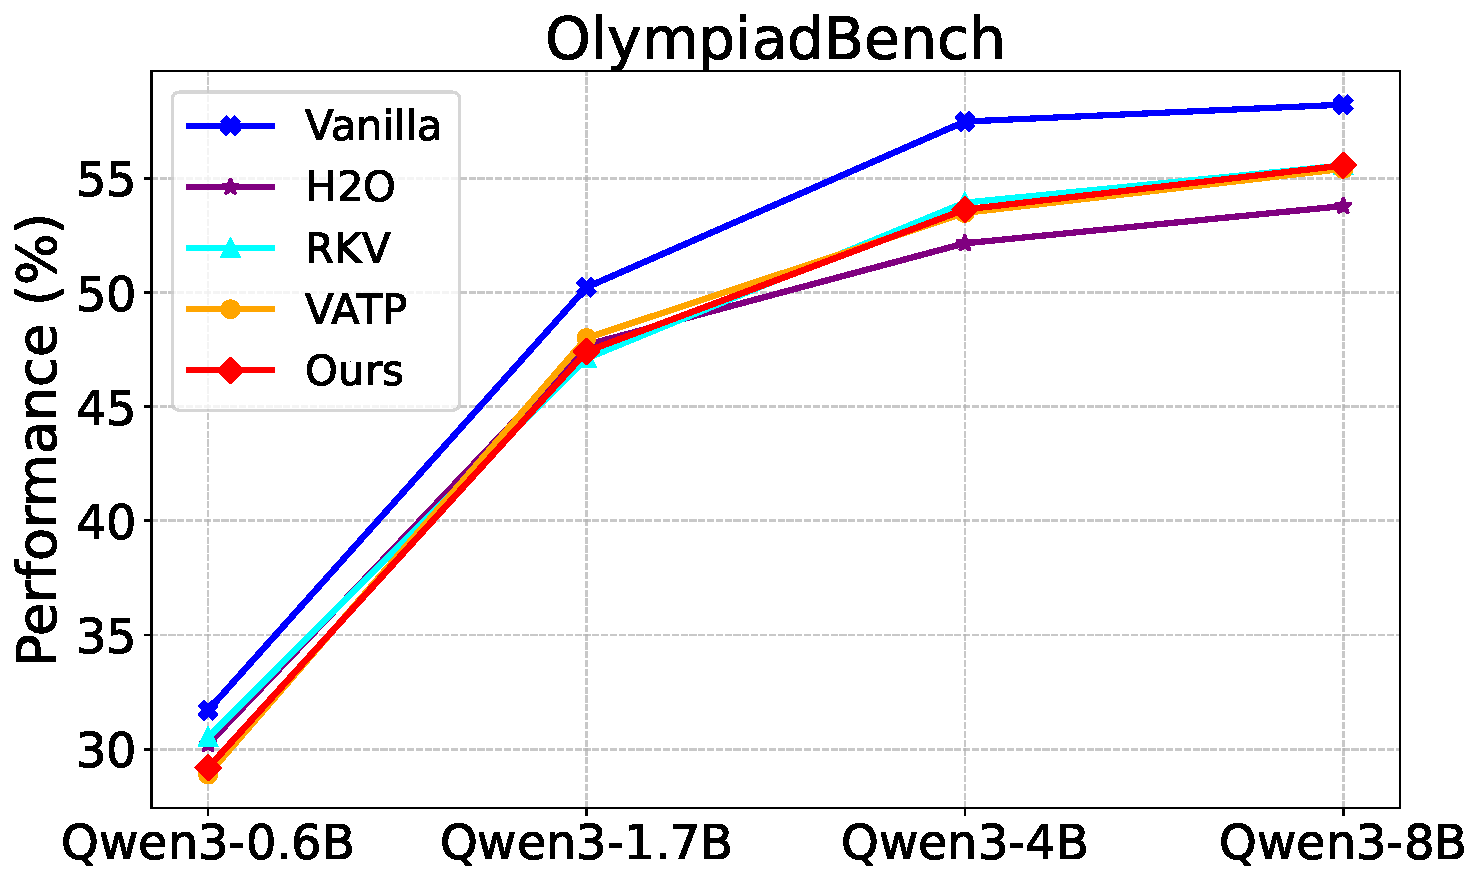
\includegraphics[width=\textwidth]{figure/experiment_different_dataset/qwen_model_OlympiadBench.pdf} % image1.png 是你的图片文件名
        % \caption{Caption for Image 1} % 子图标题 (已注释)
        \label{fig:sub1} % 子图引用标签
    \end{subfigure}
    \hfill % 在子图之间添加水平间距
    \begin{subfigure}[b]{0.32\textwidth}
        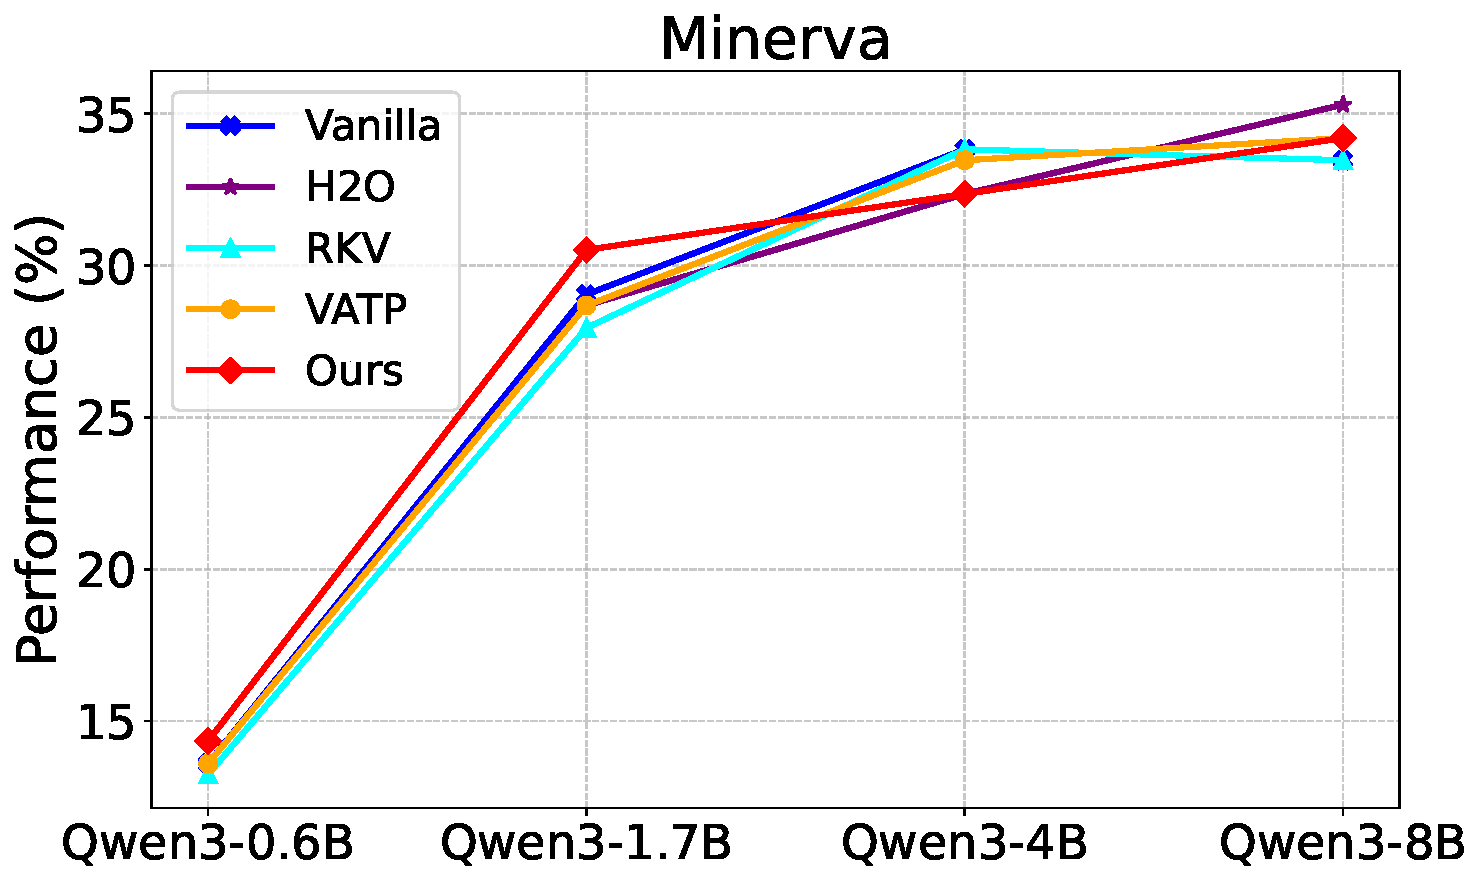
\includegraphics[width=\textwidth]{figure/experiment_different_dataset/qwen_model_Minerva.pdf}
        % \caption{Caption for Image 2}
        \label{fig:sub2}
    \end{subfigure}
    \hfill
    \begin{subfigure}[b]{0.32\textwidth}
        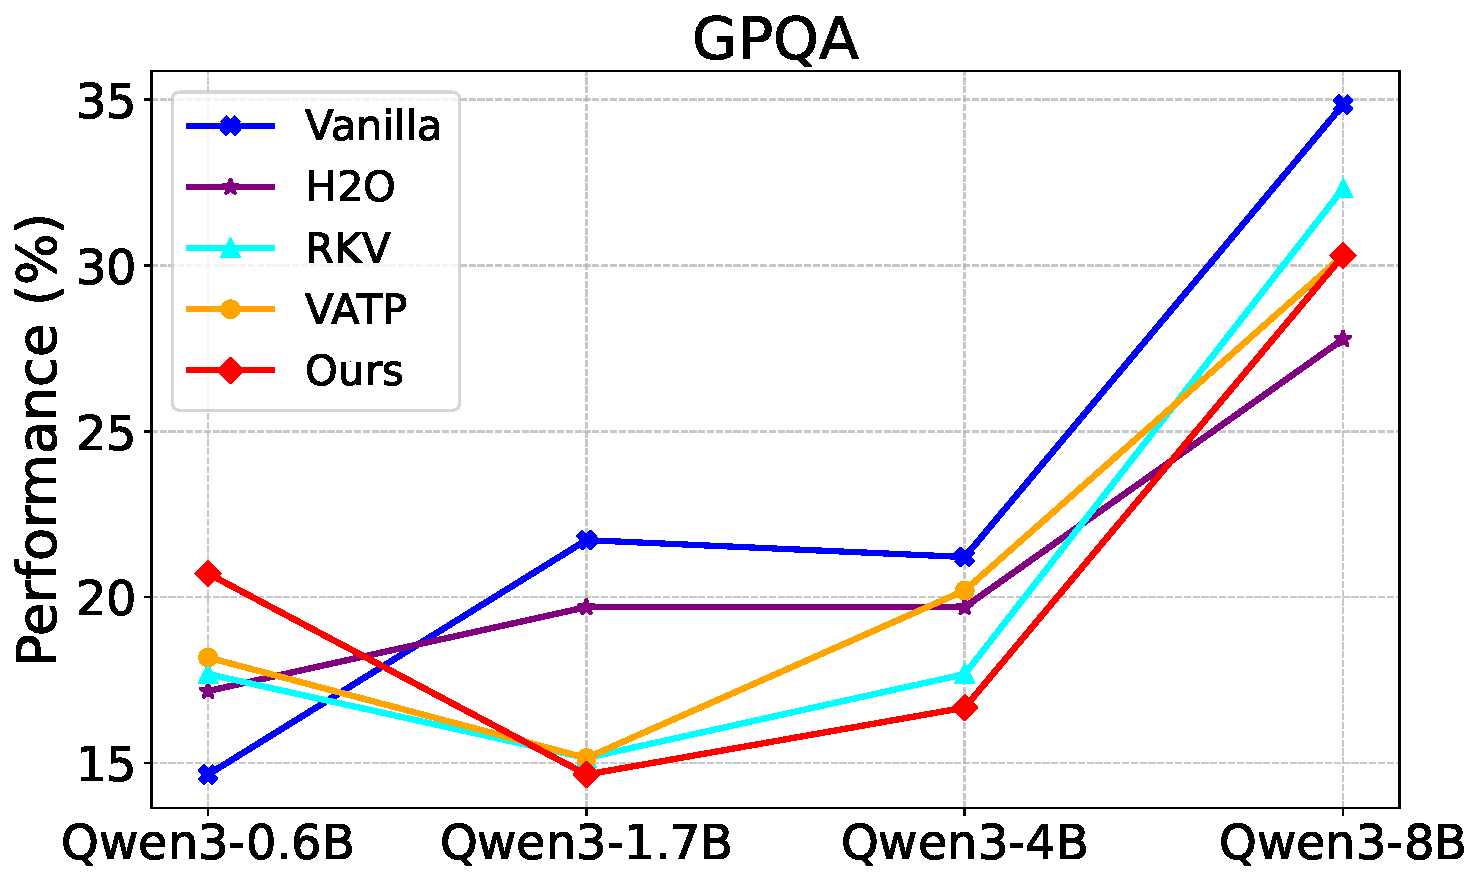
\includegraphics[width=\textwidth]{figure/experiment_different_dataset/qwen_model_GPQA.pdf}
        % \caption{Caption for Image 3}
        \label{fig:sub3}
    \end{subfigure}
    % ----------------------------------------------------------------------------------
    % 关键修改：通过负间距减少两行子图之间的垂直距离。
    % [-1.5em] 是一个常用的起始值，你可以根据实际效果调整，例如 -1em, -2em, -10pt 等。
    % ----------------------------------------------------------------------------------
    \\[-1em] 

    % 第二行
    \begin{subfigure}[b]{0.32\textwidth}
        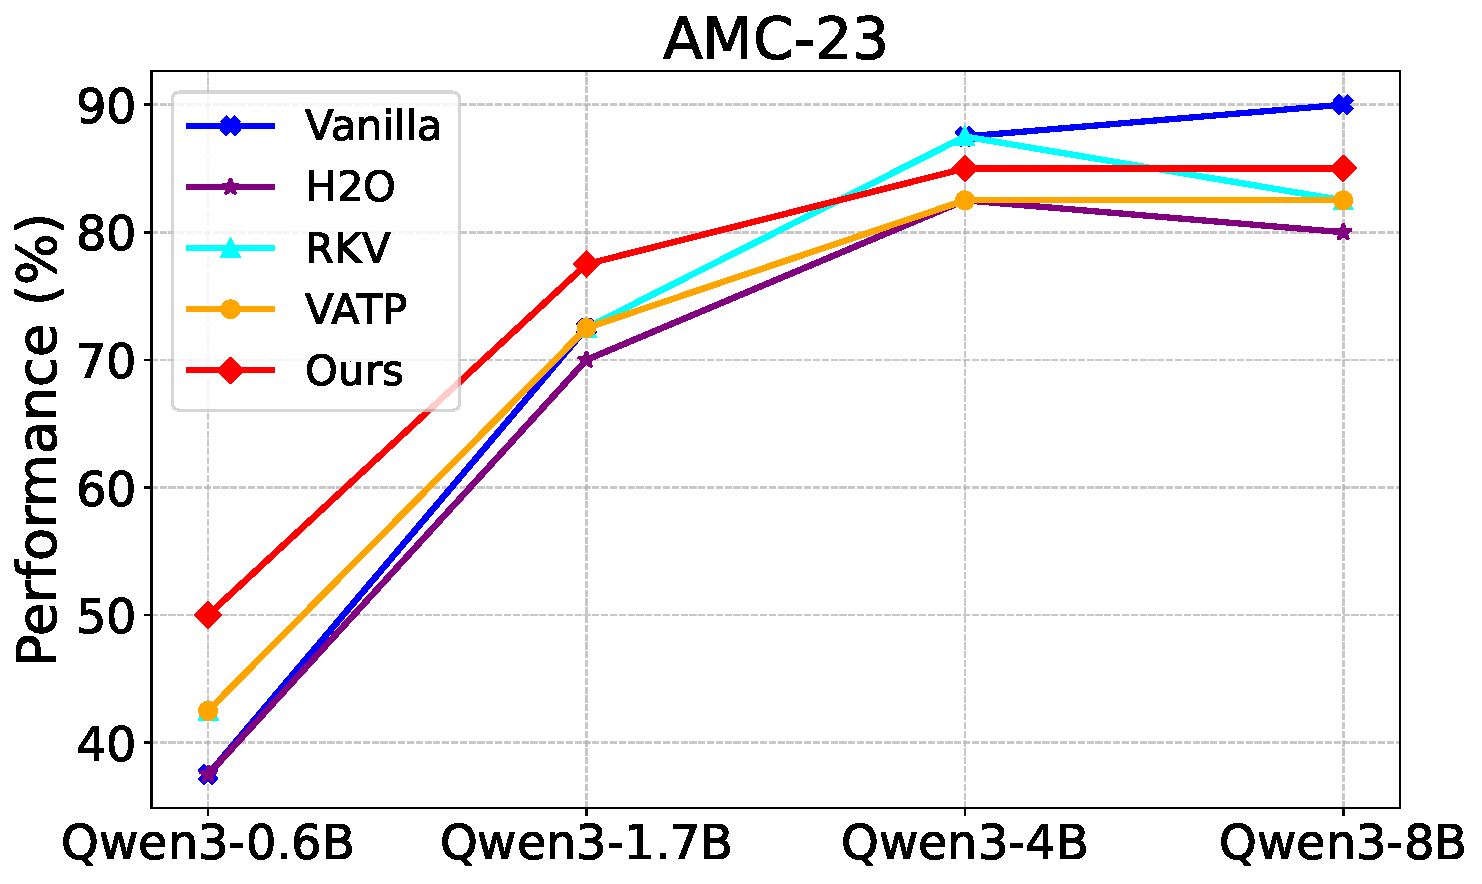
\includegraphics[width=\textwidth]{figure/experiment_different_dataset/qwen_model_AMC-23.pdf}
        % \caption{Caption for Image 4}
        \label{fig:sub4}
    \end{subfigure}
    \hfill
    \begin{subfigure}[b]{0.32\textwidth}
        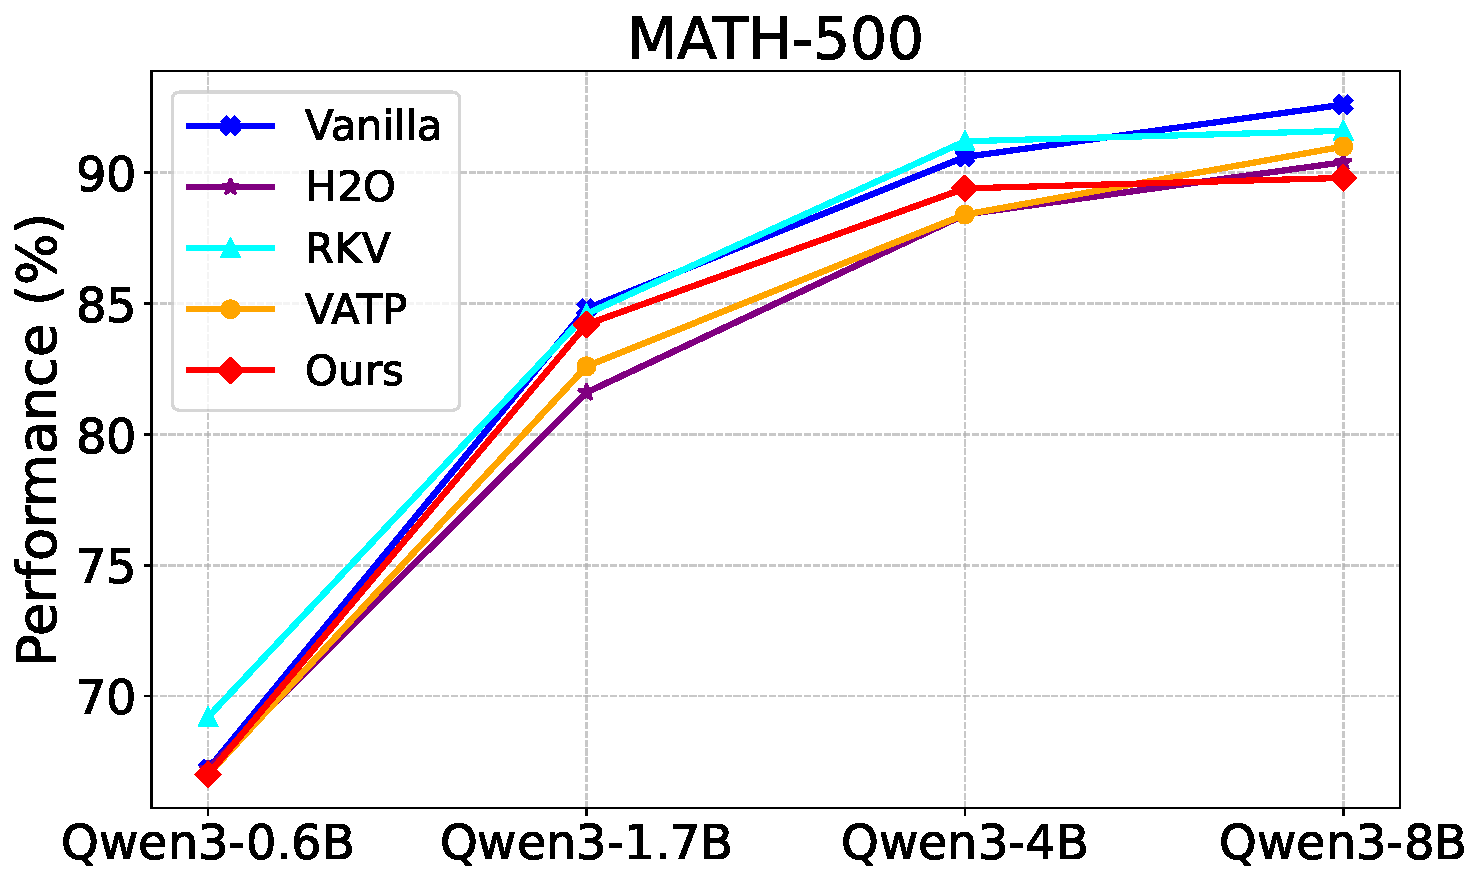
\includegraphics[width=\textwidth]{figure/experiment_different_dataset/qwen_model_MATH-500.pdf}
        % \caption{Caption for Image 5}
        \label{fig:sub5}
    \end{subfigure}
    \hfill
    \begin{subfigure}[b]{0.32\textwidth}
        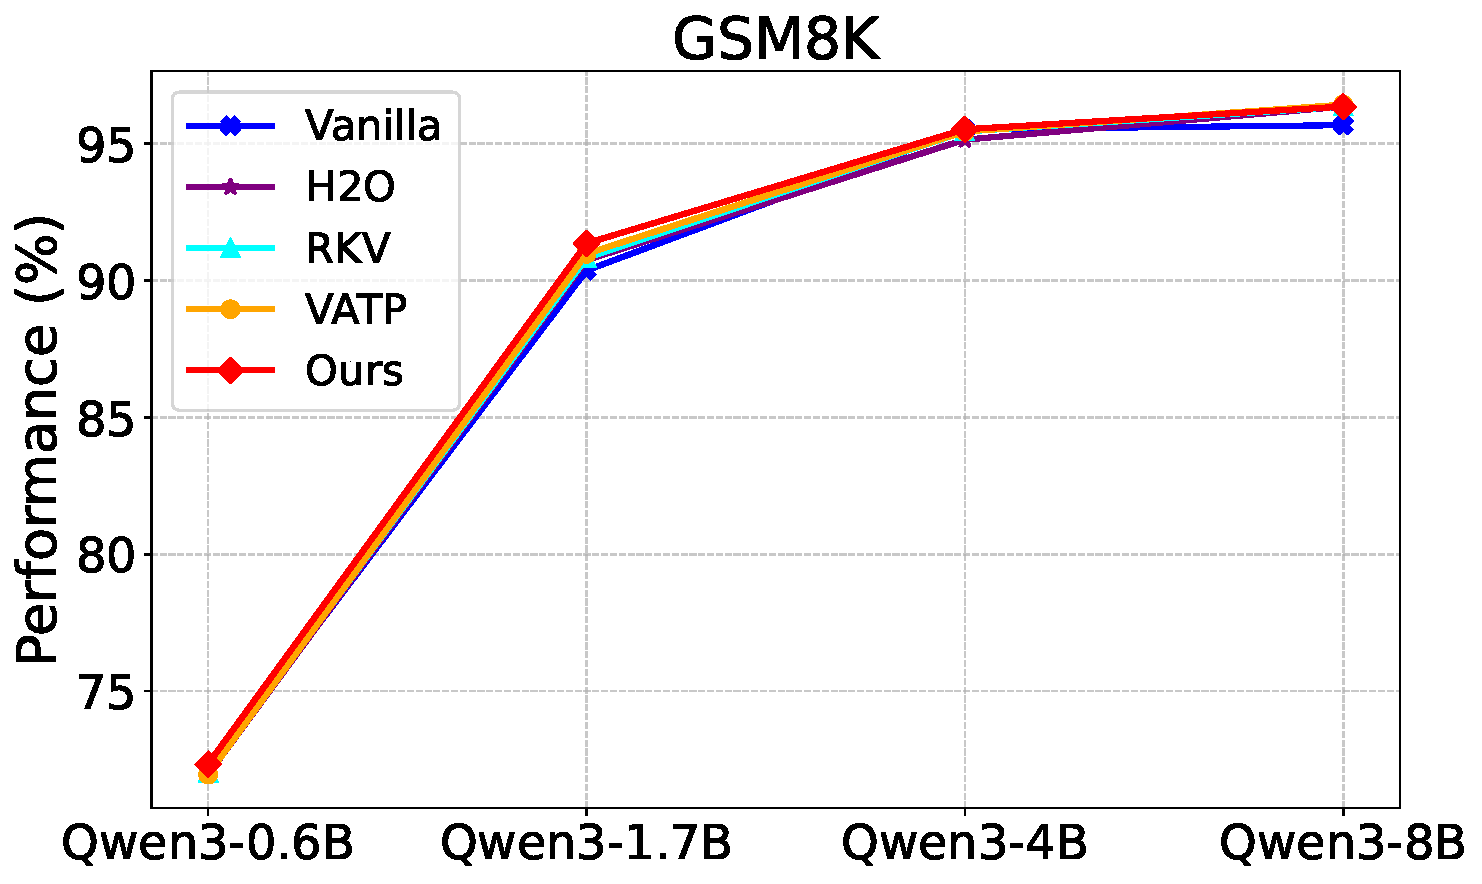
\includegraphics[width=\textwidth]{figure/experiment_different_dataset/qwen_model_GSM8K.pdf}
        % \caption{Caption for Image 6}
        \label{fig:sub6}
    \end{subfigure}
    \caption{Accuracy of LongFlow and the baselines across different model sizes on different datasets.} % 主图标题
    \label{fig:all_images} % 主图引用标签
\end{figure*}



\begin{figure*}[htbp]
    \centering
    % --- 子图 1 ---
    \begin{subfigure}[b]{0.47\textwidth} % <-- 宽度从0.48减小到0.47，增加安全边际
        \centering
        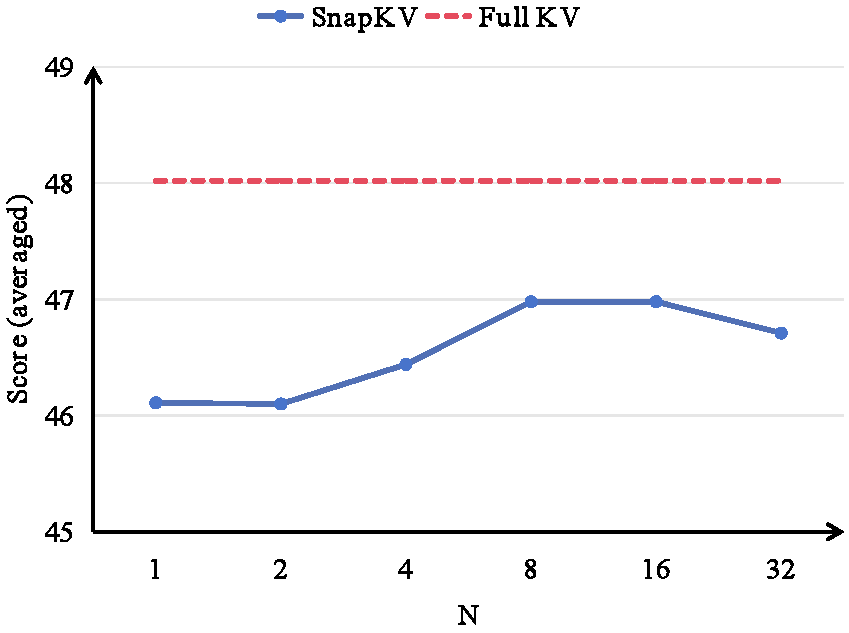
\includegraphics[width=0.8\linewidth]{figure/snap_cropped.pdf}
        \caption{SnapKV performance on LongBench as the query observation window shrinks. We use LLaMA-3-8B and an context length of 8192.}
        \label{fig:snap}
    \end{subfigure}
    %
    % --- 关键点: 上一行的 '%' 和下面这行的 '\hfill' 之间，绝对不能有任何空行 ---
    %
    \hfill
    %
    % --- 关键点: '\hfill' 和下面这行的 '\begin{subfigure}' 之间，也绝对不能有任何空行 ---
    %
    % --- 子图 2 ---
    \begin{subfigure}[b]{0.47\textwidth} % <-- 宽度从0.48减小到0.47，增加安全边际
        \centering
        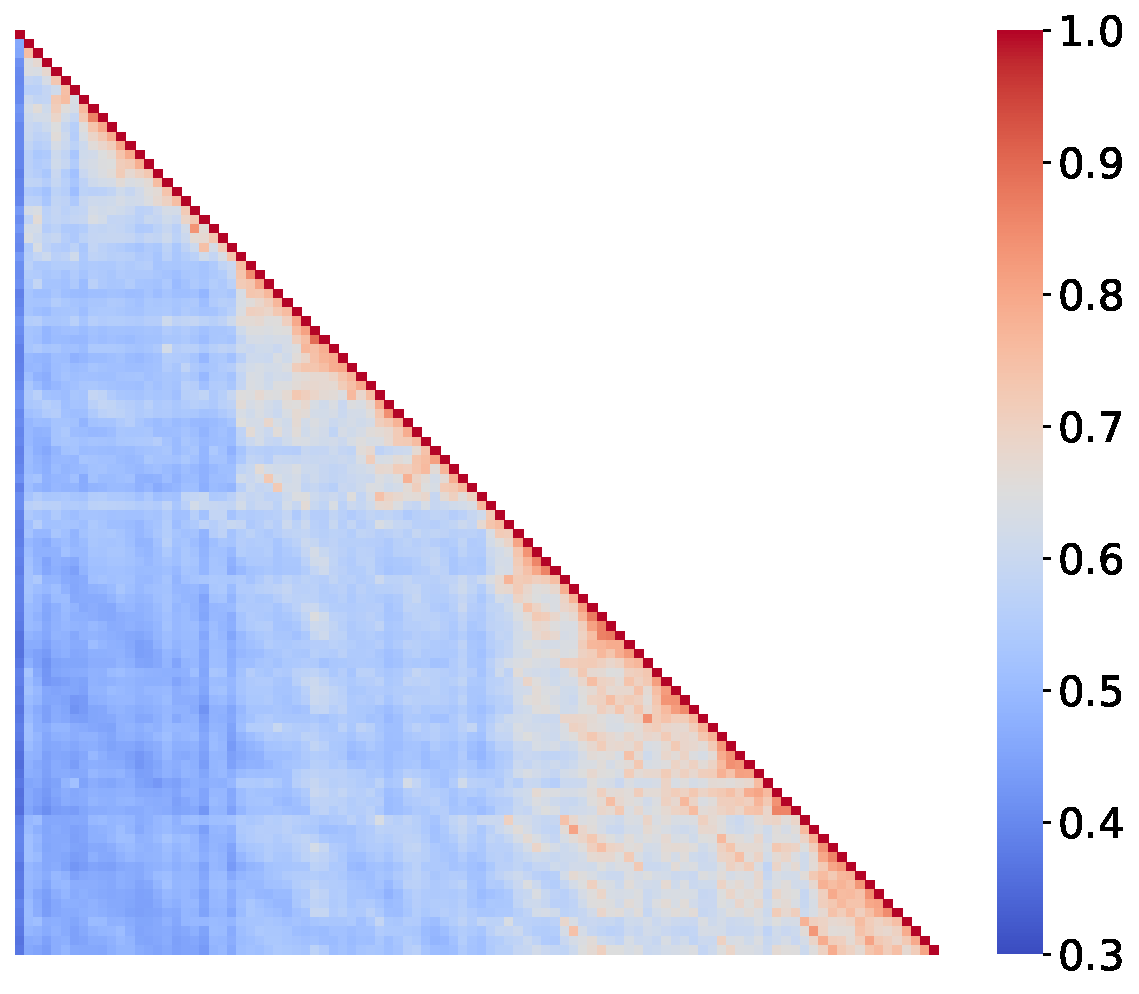
\includegraphics[width=0.8\linewidth]{figure/query_average_cosine_similarity_seqlen_100.pdf}
        \caption{Cosine similarity between queries. Results are shown for the first 100 tokens, averaged over 100 samples from MATH500 using Qwen3-8B (Layer 10, Head 10). The high and stable similarity between adjacent queries supports our approximation.}
        \label{fig:cosine_sim}
    \end{subfigure}
    
    \caption{Empirical motivation for our single-query hypothesis.}
    \label{fig:observation_figures}
\end{figure*}